%!TEX root = slides.tex

\section[Part 1]{Part 1: Evolutionary genetics of associations among
genotypes, phenotypes, and environments}

\begin{frame}
\frametitle{Definitions}
\begin{block}{Local adaptation}
\centering
Individuals of a \textbf{local} population have higher relative fitness in 
their \textbf{local} environment compared to individuals from other 
environments.
\end{block}

\begin{block}{}
\begin{itemize}
\item{Patterns in each habitat are independent of each other}
\item{Affected by gene flow}
\item{Confounded by drift, temporal sampling}
\item{Process driven by divergent selection $\longleftrightarrow$ drift}
\end{itemize}
\end{block}
\tiny
\citet{Kawecki:2004hxa}
\end{frame}


\begin{frame}
\frametitle{The genetic basis for local adaptation}
\begin{block}{Antagonistic pleiotropy vs conditional
neutrality}
\centering
\includegraphics[width=0.75\textwidth]{salvo_fig1}\\
\tiny
Adapted from \citet[Figure 1]{Savolainen:2013dfa}
\end{block}
\end{frame}


\begin{frame}
\frametitle{The genetic basis for local adaptation}
\begin{block}{Antagonistic pleiotropy vs conditional
neutrality}
\begin{itemize}
\item{AP can maintain genetic variation because of differential fitness of
loci across environments}
\item{Why hasn't AP been detected more and why is CN so abundant in the
literature?}
\end{itemize}
\end{block}
\tiny
\citet{MitchellOlds:2007di, Anderson:2012cb}
\end{frame}

\begin{frame}
\frametitle{The genetic basis for local adaptation}
\begin{block}{Is the lack of reported AP real?}
\begin{itemize}
\item{Alleles from different environments which are conditionally 
beneficial at distinct loci + levels of gene flow are low, then 
CN can contribute to LA}
\item{With gene flow recombination could create generalist 
genotypes rather than locally adapted ones}
\item{Evidence supporting CN vs AP might not be biologically based}
\end{itemize}
\end{block}
\tiny
\citet{MitchellOlds:2007di, Anderson:2012cb}
\end{frame}


\begin{frame}
\frametitle{The genetic basis for local adaptation}
\begin{block}{Is the lack of reported AP real?}
\begin{itemize}
\item{Detecting tradeoffs requires large statistical power to detect
significant fitness advantage of local alleles in 2 or more environments, 
and most studies are small}
\item{CN just may be more detectable in artificial environments b/c trade-offs
just don't happen as much as in nature}
\item{Detection of AP all but requires large field studies and careful sample
design to measure effects of local alleles across environments}
\item{Most ecologically relevant traits appear polygenic with many loci 
each having small $\alpha$}
\end{itemize}
\end{block}
\tiny
\citet{MitchellOlds:2007di, Anderson:2012cb}
\end{frame}

\begin{frame}
\frametitle{Local adaptation}
\begin{block}{In summary}
\begin{itemize}
\item{Local adaptation results from a balance between selection and gene flow
(migration)}
\item{Selection pressures can also vary spatially and temporally
(recolonization/extinction)}
\item{Phenotypic plasticity can also play a role in local adaptation, but
tough to study in trees}
\end{itemize}
\end{block}
\tiny
*Adapted from \citet{Savolainen:2013dfa}
\end{frame}

\begin{frame}
\frametitle{Methods to detect local adaptation}
\begin{block}{Current approaches*}{}
\begin{itemize}
\item{QTL-mapping}
\item{Population genetics}
\item{Association mapping}
\end{itemize}
\end{block}
\tiny
*Adapted from \citet{Savolainen:2013dfa}
\end{frame}

\begin{frame}
\frametitle{LD and marker density}
\begin{block}{How much sequencing do you need?}
\centering
\includegraphics[width=0.7\textwidth]{ld_decay}
\end{block}
\end{frame}


\begin{frame}
\frametitle{Methods to detect local adaptation}
\begin{block}{QTL}
\begin{itemize}
\item{Can operate on a reduced set of markers (GBS: RAD, ddRAD)}
\item{Does not require a reference genome}
\item{Need a linkage map, large sample sizes, many crosses}
\end{itemize}
\end{block}
\end{frame}

\begin{frame}
\frametitle{QTL in \textit{Boechera stricta}}
\begin{block}{Method to distinguish between AP and CN}
\begin{itemize}
\item{Investigate LA, ID targets of selection}
\item{Evaluates $\Delta$ in AF after selection}
\item{Using 177 $\text{F}_6$ RIL of \textit{B. stricta} and parental lines}
\item{Permutation approach, \texttt{CNAP}, using null distribution of
$\Delta_{AF}$ for all markers in all environments such that genotype is 
not related to fitness*}
\end{itemize}
\end{block}
\tiny
* Available from Corresponding author\\
\citet{Anderson:2012cb}
\end{frame}

\begin{frame}
\frametitle{QTL in \textit{Boechera stricta}}
\begin{block}{Experimental design}
\begin{itemize}
\item{Field sites in MT and CO}
\item{Relatively undisturbed, vary in elevation, latitude, precipitation and 
temperature}
\item{Signatures of selection along ecological gradients}
\item{Previous work shows substantial divergence MT and CO groups}
\item{$\text{\mars}_{\text{MT}} \times \text{\female}_{\text{CO}}$, planted in
both locations}
\item{Measured number of flowers across two growing seasons}
\end{itemize}
\end{block}
\tiny
\citet{Anderson:2012cb}
\end{frame}




\begin{frame}
\frametitle{QTL in \textit{Boechera stricta}}
\begin{columns}
\begin{column}{0.4\textwidth}
\footnotesize
\begin{block}{Flowering time}
\begin{itemize}
\item{Supports local adaptation due to favored native alleles at 
both sites($\bar{\Delta} f_C = 0.016, \bar{\Delta} f_M = 
0.048, p < 0.001$)}
\item{2.8\% of genome is AP, 8.1\% CN}
\item{$\sim$all AP linked to \textit{nFT}}
\end{itemize}
\end{block}
\end{column}
\begin{column}{0.6\textwidth}
\centering
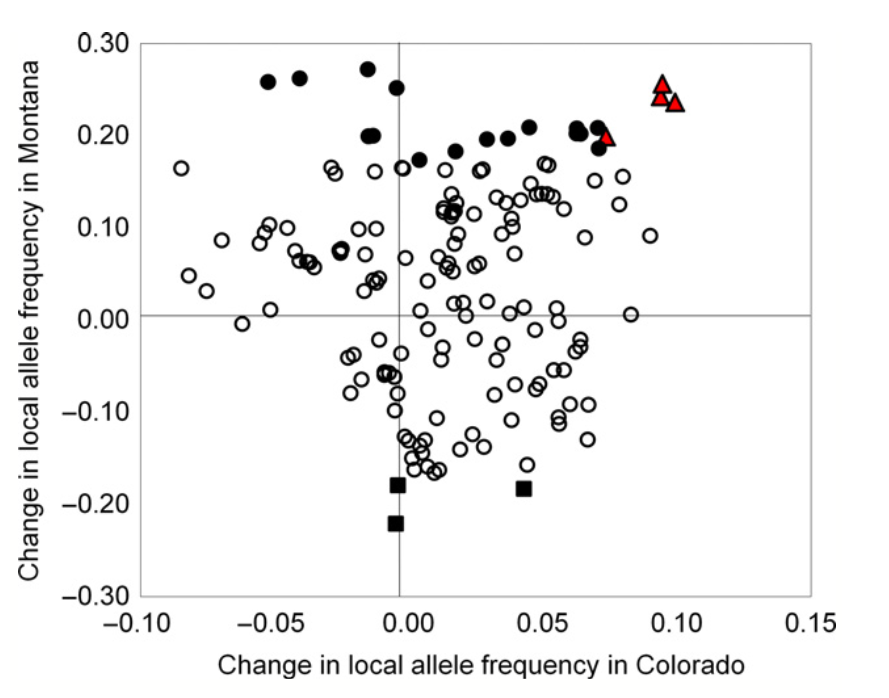
\includegraphics[width=0.9\textwidth]{boechera.png}\\
\tiny
Adapted from \citet[Figure 1]{Anderson:2012cb}
\end{column}

	
\end{columns}

\end{frame}

\begin{frame}
\frametitle{QTL in \textit{Boechera stricta}}
\begin{block}{\textit{nFT QTL $\times$ E}}
\centering
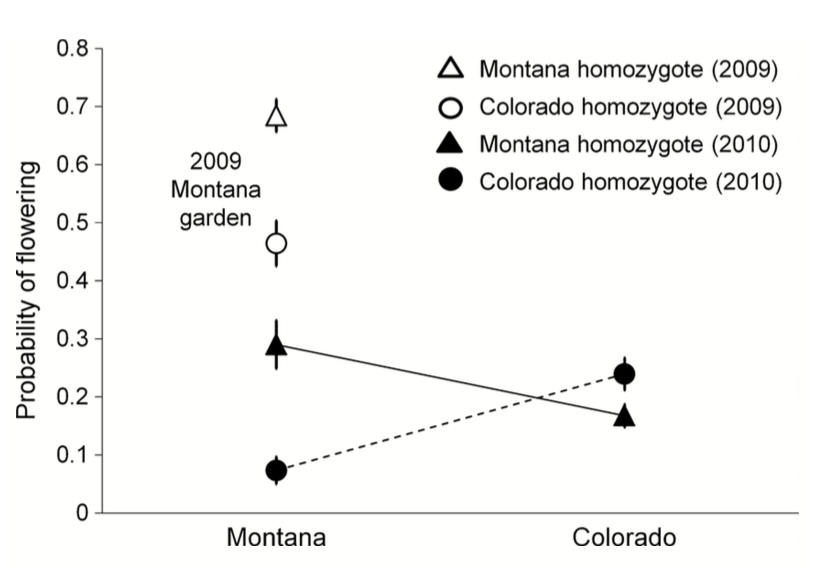
\includegraphics[width=0.7\textwidth]{boechera2.png}\\
\tiny
Adapted from \citet[Figure 3]{Anderson:2012cb}
\end{block}
\end{frame}

\begin{frame}
\frametitle{Methods to detect local adaptation}
\begin{block}{Population genetics}
\begin{itemize}
\item{Diverse data sets (SNPs, microsatellites): DNA sequence variation,
$F_{ST}$, $Q_{ST}$}
\item{Conculsions driven by data type}
\item{Requires a reference genome}
\item{Normal challenges of next-gen data apply (quality filtering, redundancy,
coverage)}
\end{itemize}
\end{block}
\end{frame}


\begin{frame}
\frametitle{Methods to detect local adaptation}
\begin{block}{Association Mapping}
\begin{itemize}
\item{Marker density depends on LD decay $\uparrow$ LD decay $\rightarrow$
$\uparrow$ marker density}
\item{$\downarrow$ LD  $\rightarrow$ $\uparrow$ marker density}
\item{Rare SNPs may be missed with small sample sizes}
\item{Genomic or exonic; careful when genome size is $\uparrow$ and LD is
$\downarrow$}
\end{itemize}

\end{block}
\end{frame}

\begin{frame}
\frametitle{Methods to detect local adaptation}
\begin{block}{Association Genetics in Douglas Fir \citep{Eckert:2009hha}}
\begin{itemize}
\item{384 SNPs (117 candidate genes), 21 cold-hardiness traits}
\item{Cold-hardiness also synchronized with photoperiod and temperature}
\item{adaptive genetic diversity segregates along environmental gradients}
\end{itemize}
\end{block}
\end{frame}

\begin{frame}
\frametitle{Methods to detect local adaptation}
\begin{block}{Cold-hardiness traits}
\centering
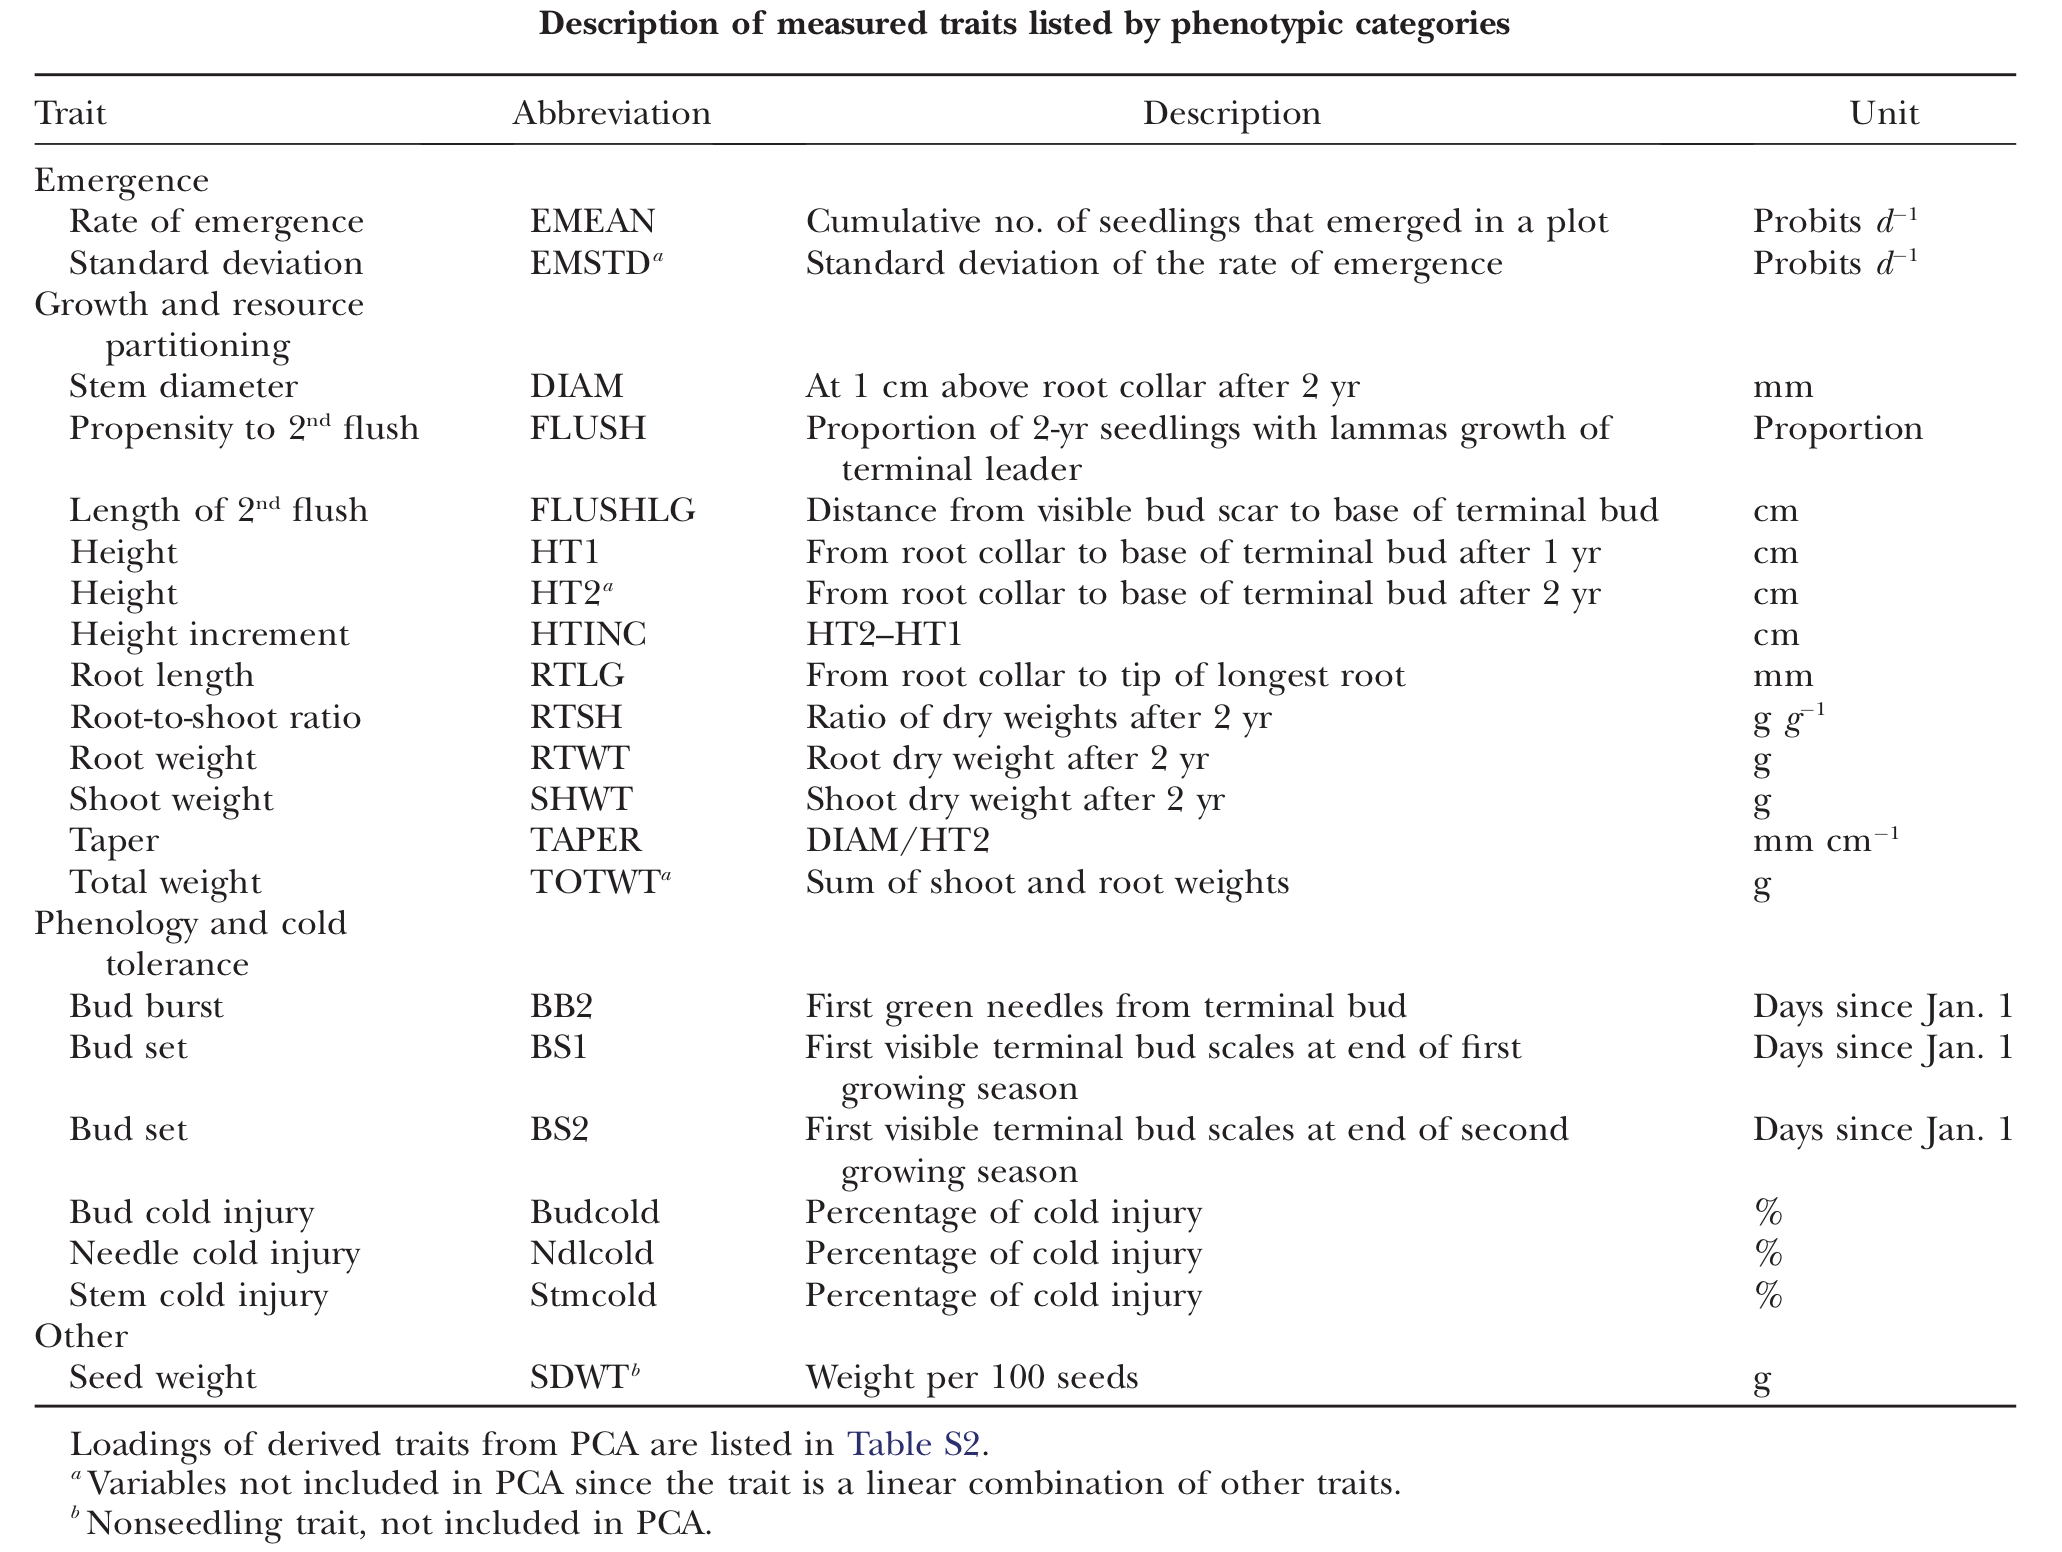
\includegraphics[height=0.8\textheight]{eckert2.png}
\end{block}
\end{frame}


\begin{frame}
\frametitle{Methods to detect local adaptation}
\begin{block}{}
\begin{centering}
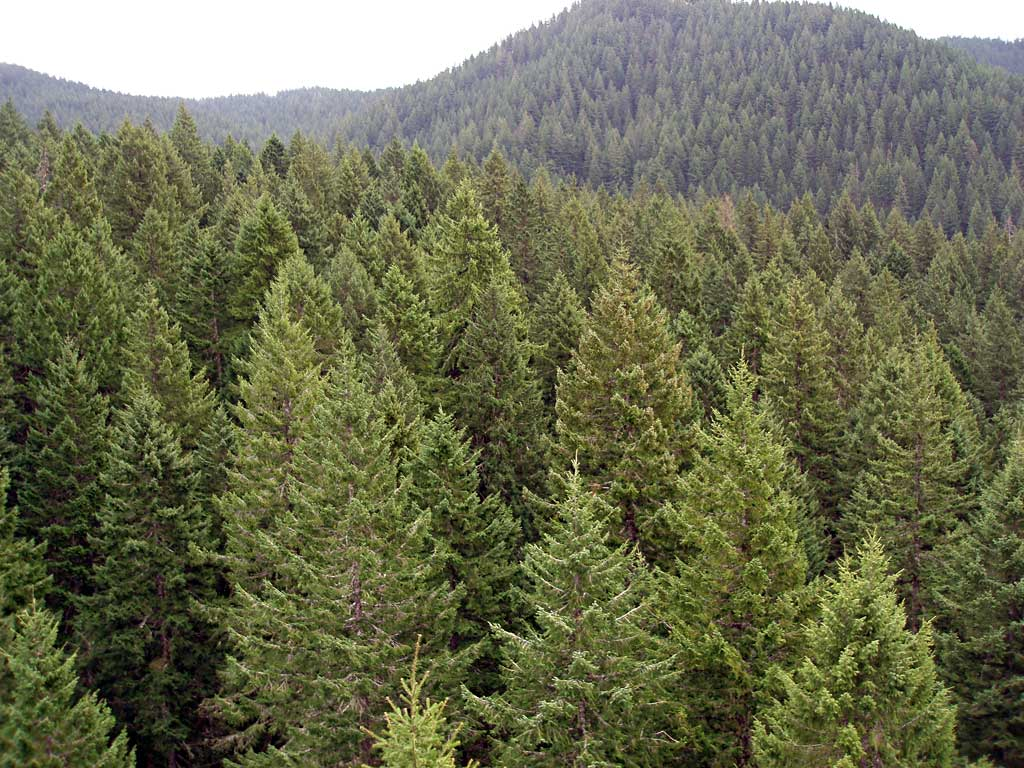
\includegraphics[height=0.5\textheight]{dougfir.jpg}
\hspace{1em}
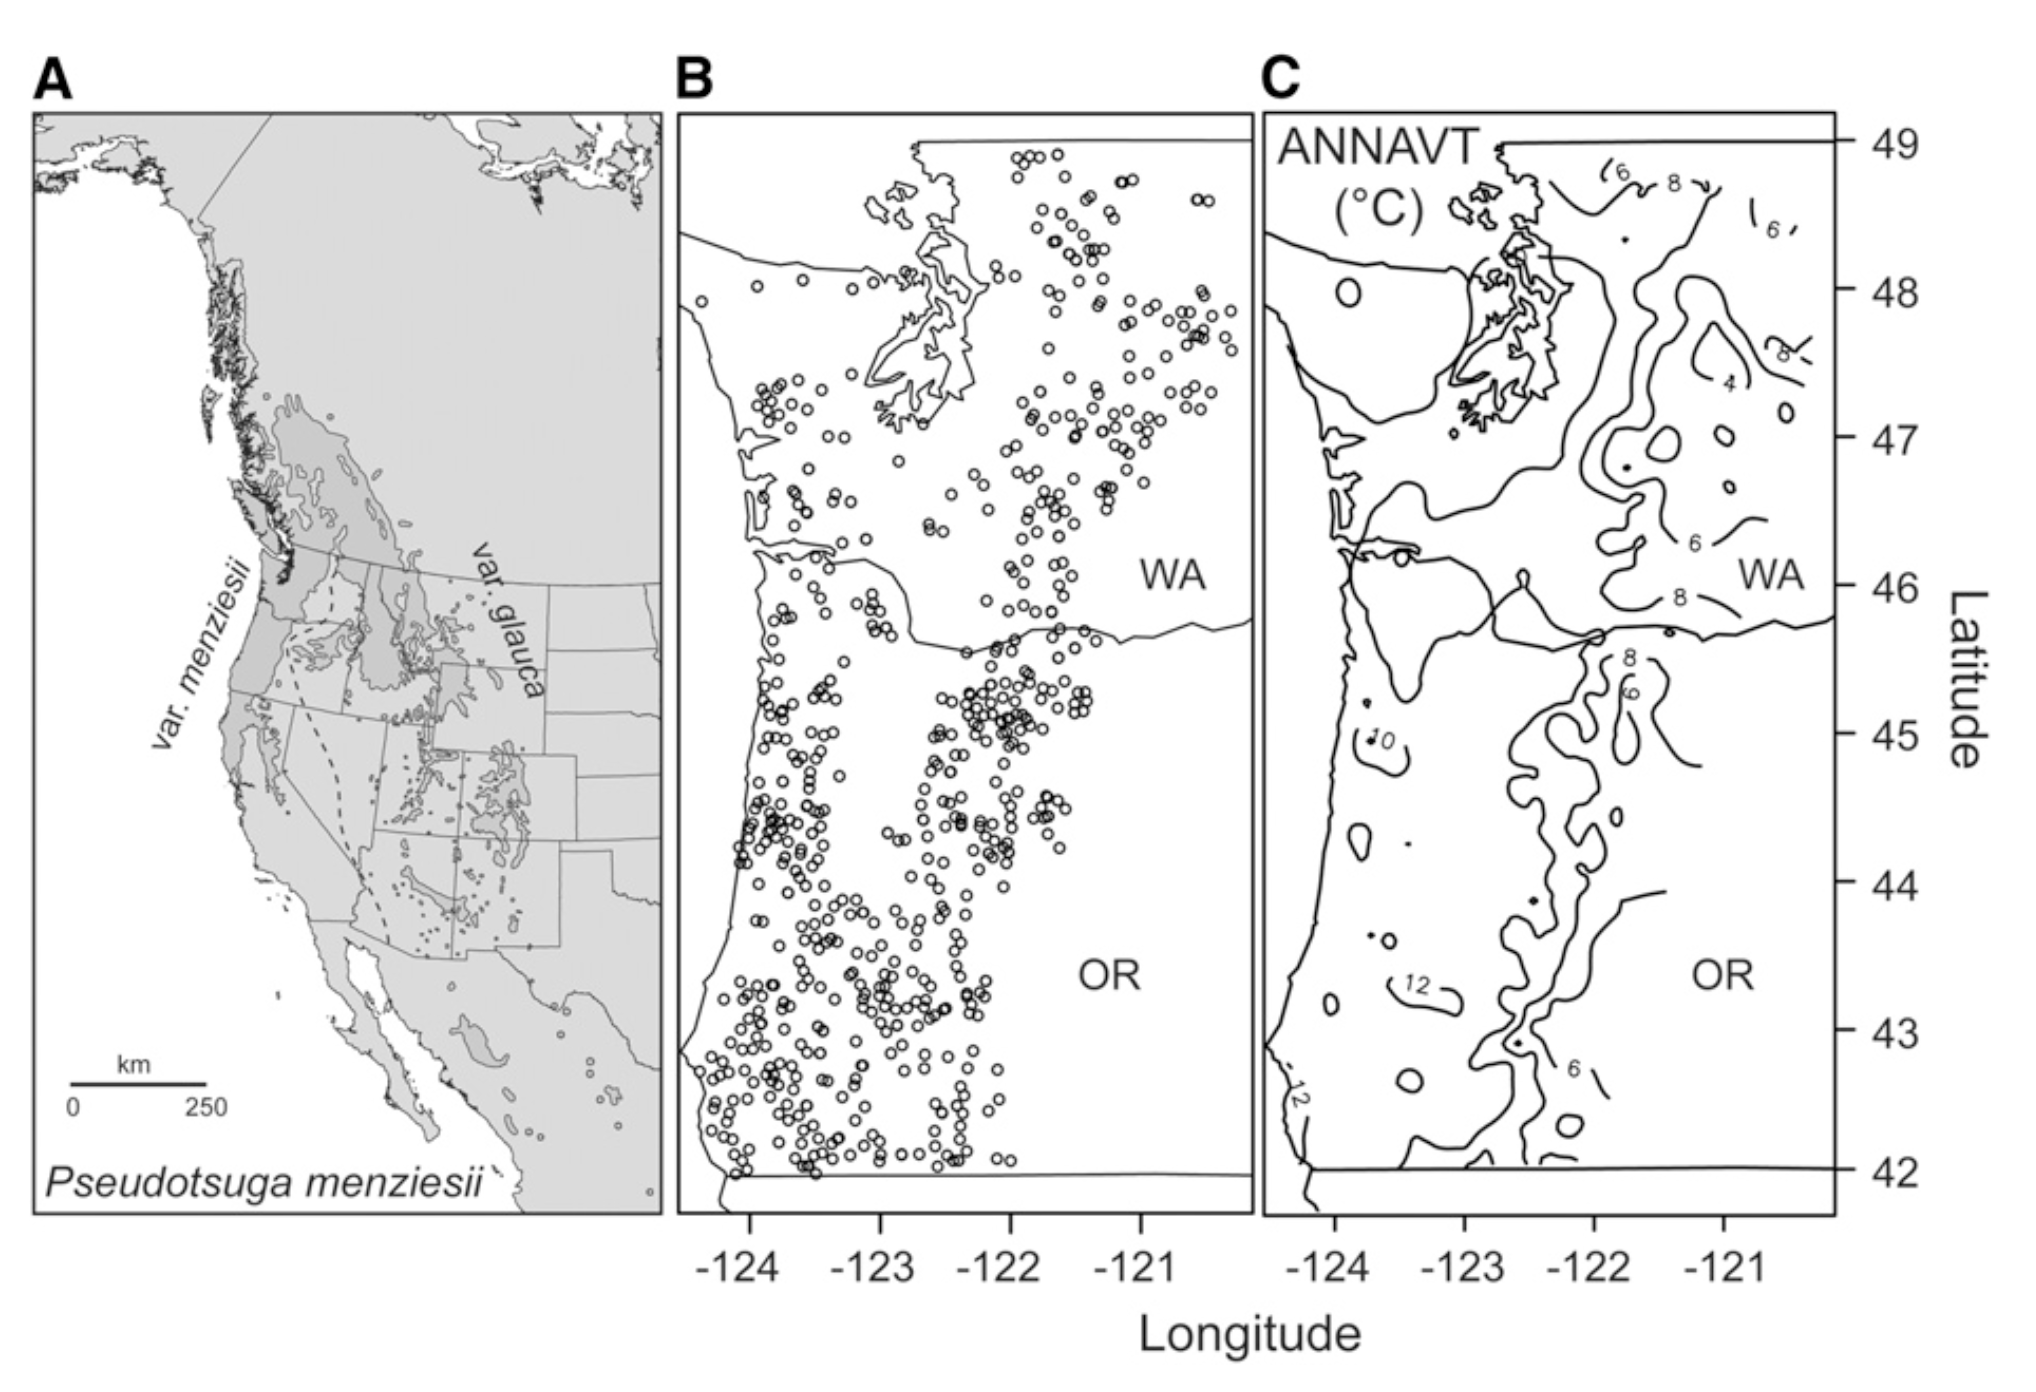
\includegraphics[width=0.45\textwidth]{eckert1.png}
\end{centering}
\begin{itemize}
\item{Haploid tissue sampling (10 megs/tree)}
\item{GoldenGate SNP array}
\item{\citet{Yu:2006ij, Storey:2003wo}, $\text{AMOVA}_{hier}$, Tassel}
\end{itemize}
\end{block}
\end{frame}

\begin{frame}
\frametitle{Methods to detect local adaptation}
\begin{block}{Results}
\begin{itemize}
\item{Low population structure ($G_{ST} \sim 0.02--0.07$), $Q$-matrix of k=15
from STRUCTURE}
\item{455 (p < 0.05); 30 (q < 0.1); of the 30, 15 unique SNPs from 12
candidate genes, affecting 10 different traits}
\item{Growth/resource: 4 associations in 4 genes}
\item{Phenology/cold-tolerance: 18 assoc, 11 unique snps, 10 candidate genes. 
Man of these were non-additive}
\item{Multivariate phenotypes: PC1 $\sim$ 44.8\%;  PC1 =
growth+phenology+cold-tolerance, PC2 = cold damage}
\item{individual SNPs only account for small \% of phenotypic variance}
\item{Most of genes with significant associates to at least one trait (n =
13) have action other than codominance.}
\end{itemize}
\end{block}
\end{frame}




\begin{frame}
\frametitle{Evolutionary quantitative genetics}
\begin{block}{}
\centering
\includegraphics[height=0.8\textheight]{sork}\\
\tiny
Adapted from \citet[Figure 1]{Sork:2013tb}
\end{block}{}
\end{frame}

\begin{frame}
\frametitle{Evolutionary quantitative genetics}
\begin{block}{Goals}
\begin{itemize}
\item{Understand the genetics and inheritance of complex traits}
\item{Nature and strength of evolutionary forces}
\item{Natural populations}
\end{itemize}
\end{block}

\begin{block}{Natural selection}
\begin{itemize}
\item{On traits}
\item{Heritability}
\item{Variation/Variance}
\item{Additive genetic variation}
\end{itemize}
\end{block}
\tiny
\citet{Walsh:2008}
\end{frame}

\begin{frame}
\frametitle{The data we have is from multiple sources}
\begin{block}{Our data}
\begin{itemize}
\item{A sampling of individuals}
\item{A sampling of populations made up of those individuals}
\item{Some genetic data from these individuals}
\item{Some phenotypic data about the individuals}
\item{Some data about the populations (e.g., location)}
\end{itemize}

\end{block}\end{frame}

\begin{frame}
\frametitle{There are several things we'd like to do with our data}

\begin{block}{Genetic architecture}
\begin{itemize}
\item{Ascertain a meaningful set of genetic variants which sufficient
discriminatory power}
\item{Use this genetic variation to understand something about the 
traits of the organism we care about}
\item{In other words, given a set of traits that we observe in nature, and as
scientists we find interesting, can we attribute variation in that trait with
variation in the genome}
\end{itemize}
\end{block}
\end{frame}

\begin{frame}
\frametitle{There is some math we need}
\begin{block}{}
\begin{equation}
\label{eqn:V_P}
V_P = V_G + V_E + V_{GE}
\end{equation}

\begin{equation}
\label{eqn:V_G}
V_G = V_A + V_D + V_I
\end{equation}

\begin{equation}
\label{eqn:V_A}
V_A = 2pq\alpha^2
\end{equation}

\begin{equation}
\label{eqn:alpha}
\alpha = a + d(q-p)
\end{equation}

\begin{equation}
\label{eqn:a}
a = \frac{G_{AA}-G_{aa}}{2}
\end{equation}

\begin{equation}
\label{eqn:d}
d = G_{Aa} - \frac{G_{AA}+G_{aa}}{2}
\end{equation}

\end{block}{}
\end{frame}

\begin{frame}
\frametitle{Variance components}
\begin{block}{Equation \ref{eqn:V_P}: $V_P = V_G + V_E + V_{GE}$}
\begin{itemize}
\item{$V_P$: Phenotypic variance ($\sigma^2_P$)}
\item{$V_G$: Genetic variance}
\item{$V_E$: Environmental variance}
\item{$V_{GE}$: Genetic*environment}
\end{itemize}
\end{block}
\end{frame}

\begin{frame}
\frametitle{Genetic variance}
\begin{block}{Equation \ref{eqn:V_G}: $V_G = V_A + V_D + V_I$}
\begin{itemize}
\item{$V_G$: Total genetic variance}
\item{$V_A$: Additive genetic variance}
\item{$V_D$: Dominance genetic variance}
\item{$V_I$: Epistatic genetic variance (I = interaction)}
\end{itemize}
\end{block}
\end{frame}

\begin{frame}
\frametitle{Additive gentic variance}
\begin{block}{}
\begin{itemize}
\item{Contribution of these alleles to a phenotype are independent of 1) other
genes and 2) the environment}
\item{When multiple alleles contribute to a single phenotype (polygenic), their
presence has a linear effect on the phenotype}
\item{$V_A$ is the target of natural selection}
\end{itemize}
\end{block}{}
\end{frame}

\begin{frame}
\frametitle{Heritability}
\begin{block}{The Breeder's equation}
\begin{center}
\huge
$R = h^2S$
\end{center}
\begin{itemize}
\item[]{$R$: response to selection}
\item[]{$h^2$: narrow sense heritability ($\frac{V_A}{V_P}$)}
\item[]{$S$: selection coefficient}
\end{itemize}
\end{block}

\begin{block}{Example}
\href{http://localhost:8888/notebooks/heritability.ipynb}{heratibility.ipynb}
\end{block}
\end{frame}






\begin{frame}
\frametitle{Methods to detect local adaptation}
\begin{block}{Association Mapping}
\begin{itemize}
\item{Sampling from populations}
\item{Much lower LD among loci}
\item{Needs dense sets of markers (varies with LD and genome size)}
\item{Must consider genetically differentiated populations, population
structure is important!}
\end{itemize}
\end{block}
\end{frame}

\begin{frame}
\frametitle{Association mapping in conifers}
\begin{block}{GWAS in trees}
\begin{itemize}
\item{Forest trees are important economically and environmentally}
\item{Studying them in traditional ways (i.e., QTL) is difficult: generation
time is long, phenotype not present in seedlings (e.g, wood/bark)}
\item{Complex demography, population structure, local adaptation can confound 
associations}
\item{Heritability tends to be low for traits of interest}
\item{Mapping populations may not generalize to natural populations}
\end{itemize}
\end{block}
\tiny
\citet{Uchiyama:2013ci}
\end{frame}

\begin{frame}
\frametitle{Association mapping in conifers}
\begin{block}{Conifer genomes}
\begin{itemize}
\item{Huge: \SIrange{10}{30}{GB}}
\item{Highy complex (repeats, gene content, GC-bias)}
\item{Ratio of genetic to physical distance $>$\SI{3000}{kb \per cM}}
\item{Rapid decay of LD in coding regions}
\end{itemize}
\end{block}
\tiny
\citet{Uchiyama:2013ci,Hirschhorn:2005cka}
\end{frame}

\begin{frame}
\frametitle{Association mapping in conifers}
\begin{block}{Identifying variants}
Two main methods:
\begin{itemize}
\item{Genotyping arrays}
\item{Gentoyping by sequencing (GBS)}
\item{Each have own set of biases and problems}
\end{itemize}
\end{block}
\end{frame}

\begin{frame}
\frametitle{Now that you have identified variants...}
\begin{block}{Let's revisit what you want to do}
\centering
You want to understand how the variation in your biologically important and
interesting trait is attributable to the underlying additive genetic variation 
present (i.e., heritability) in your samples (and hopefully the population).
\end{block}
\end{frame}

